\chapter{Radiative corrections}
\label{radiative}

The radiative corrections were done using new double-pion event generator (see Iu. Skorodumina wiki page~\cite{Skorodum:EG} and Sect~\ref{eff_aval}). For that purpose double-pion events were generated with and without radiative effects.  After that radiative
correction factor $R$ in formula~(\ref{expcrossect})
was determined as:
\begin{equation}
\label{radcorrfact}
R = \frac{N_{rad}^{2D}}{N_{norad}^{2D}} \textrm{ ,}
\end{equation}
where $N_{rad}^{2D}$ and $N_{norad}^{2D}$ are
numbers of generated events in each $(W, Q^{2})$ bin
with and without radiative effects.
Quantity one over $R$ is plotted in the left side of Fig.~\ref{radcorrfact} as function of $W$ for various $Q^{2}$ bins. As it seen from Fig.~\ref{radcorrfact} dependence of the radiative correction factor on $Q^{2}$ is rather small. So, in actuall cross sections calculations factor $R$ averaged over all $Q^{2}$ bins was used (see right side of Fig.~\ref{radcorrfact}). Statistical uncertainties associated with number of generated events are also small and not seen on Fig.~\ref{radcorrfact}.

\begin{figure}[htp]
\begin{center}
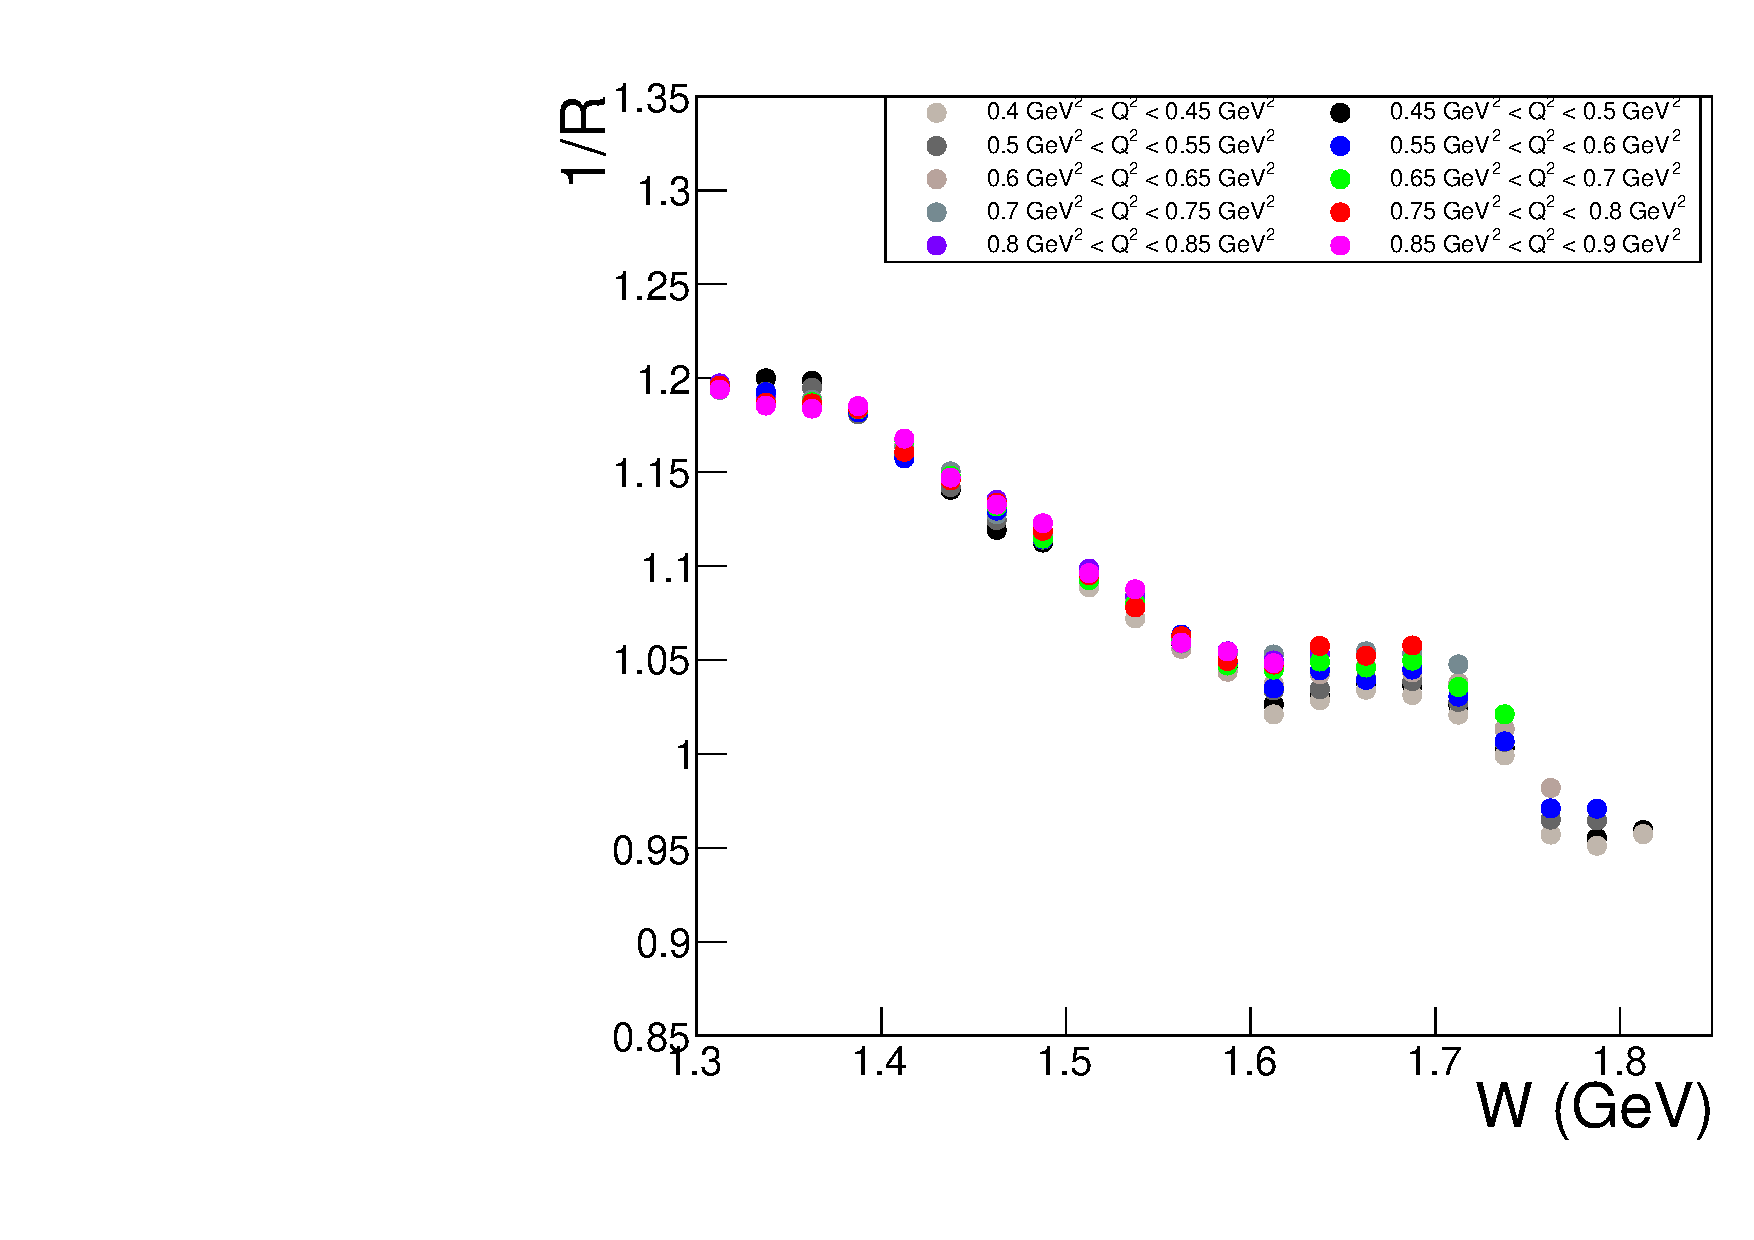
\includegraphics[width=8cm]{pictures/rad_corr/rad_corr_all_q2.pdf}
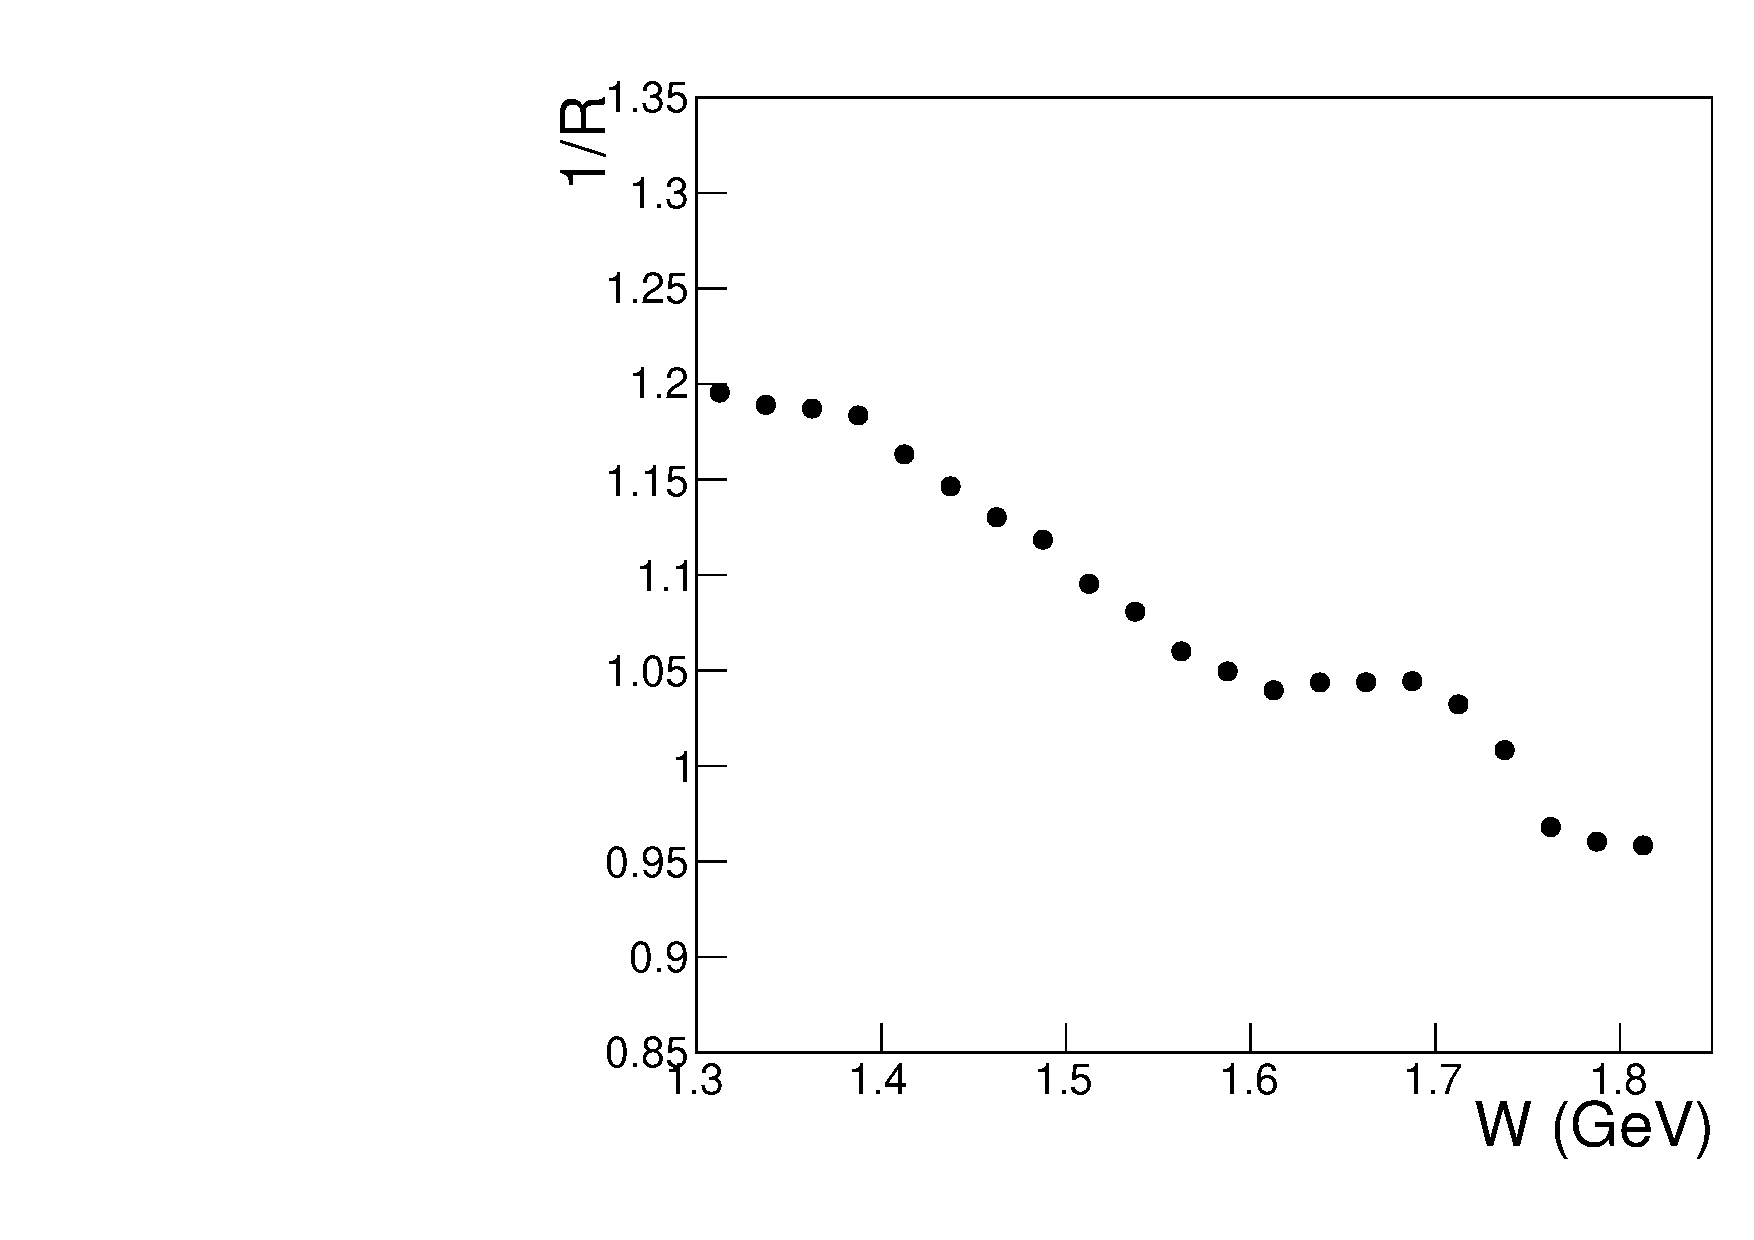
\includegraphics[width=8cm]{pictures/rad_corr/rad_corr_avrg.pdf}
\caption{\small One over radiative correction factor (see formula~\ref{expcrossect})
as function of $W$, for various bins over $Q^{2}$ (left plot) and averaged over all  $Q^{2}$ bins (right plot).} \label{radcorrfact}
\end{center}
\end{figure}

It should be noted that to account for radiative effects new double-pion event generator uses well
known approach taken from Mo and Tsai paper~\cite{Mo:1968cg}.
In this approach soft part is evaluated
explicitly, while for calculation of the hard part "inclusive" hadronic
tensor is used. An applicability
of such approximation for hard part of
radiative effects is the subject of special
attention. The single-differential double-pion cross sections~(\ref{inegr5diff}) obtained in this analysis represent integrated over four
variables five-differential cross section. This
integration considerably reduces the influence of
the final hadron kinematics on
radiative correction factor. So,
"inclusive" Mo and Tsai procedure in the case of double-pion cross sections  looks more
applicable than in a case
of non-integrated cross sections that are typically obtained for instance in single pion data analysis.
